

%\subsubsection{Dans un noeud}
\SbSbSSCT{Dans un noeud}{In a node}

 \begin{tabular}{|c | c | } \hline
 \begin{tikzpicture}[baseline=0pt]
 \draw (0,0) grid (4,3);
 \node [fill=green!20,trapezium,draw] at (1,2) {\DFR};
 \node  [draw] at (3,1) {
\includegraphics[width=1cm]{tiger} };
 \end{tikzpicture} 
 &
  \parbox[b]{10cm}{
  \BS{begin}\AC{tikzpicture}   \\
   \BS{draw} (0,0) grid (5,3); \\
  \BS{node} [fill=green!20,trapezium,draw] at (1,2) \AC{\BS{DFR} }; \pageref{DFR} \\
\BS{node}  [draw] at (3,1) \AC{\BS{includegraphics}[width=1cm]\AC{tiger} };\\
  \BS{end}\AC{tikzpicture}
 }
   \\  \hline
  \end{tabular}
  
 
 
%\subsubsection{En déclarant l'image dans pgf}
\SbSbSSCT{En déclarant l'image dans pgf}{With pgfdeclareimage}


 \begin{tabular}{|c | c | } \hline
 \pgfdeclareimage[width=3cm]{ttt}{tiger}
% \pgfuseimage{tiger}
 
 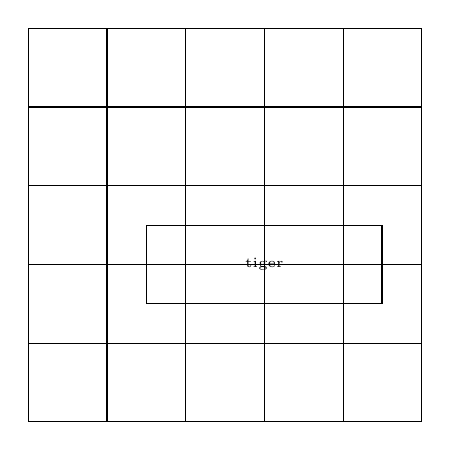
\begin{tikzpicture}[baseline=1cm]
 \draw (0,0) grid (5,5);
\draw (3,2) node {\pgfuseimage{ttt}} ;
 \end{tikzpicture} 
 &
 \parbox[b]{8cm}{
  \BSS{pgfdeclareimage}[width=3cm]\AC{ttt}\AC{tiger}\\
\\
\\  
  \BS{begin}\AC{tikzpicture}\\
  \BS{draw} (0,0) grid (5,5); \\
  \BS{draw} (3,2) node \AC{\BSS{pgfuseimage}\AC{ttt}} ; \\
  \BS{end}\AC{tikzpicture}
 }
  \\  \hline
 \end{tabular}
 